%----------------------------------------------------------------------------------------
%	CLASSIFICATION OF DATA VIA DIFFERENT METHODS
%
%	Classification of the data using different approaches.
%----------------------------------------------------------------------------------------
\section{Classification}

Given the structure of our dataset, namely image data with a sub dataset with corresponding class labels, and a sub dataset with corresponding feature labels, different machine learning and computer vision methods were chosen, to tackle the problem of image classification. \\
\\
Image classification refers to the method of identifying to which category an image belongs to, according to its visual information.  Classification problems can be divided into three different types: binary, multi-class and multi-label. Whereas a binary classification only distinguishes between two different classes and therefore classifies an image into one of the two classes, a multi-class classification distinguishes between multiple exclusive classes. A multi-label classification also works for multiple classes. However, a single image can belong to none, one, several or all of the classes. Those classes can be seen as a feature vector for each image. Each feature can be present or not, independently of the other features ( vielleicht hier zitieren, seite muss noch rausgesucht werden)~\citep{har2003constraint}. \\

Each of those classification methods comes with certain advantages and implications.
There exist many classification methods which have been developed for binary classification problems, but less methods are suited for multi-label or multi-class classification. Therefore, the latter often work as a combination of binary classifiers. Moreover, multi-class and multi-label classification have the difficulty of sparser labels. \\

Binary classification can be used to decide whether a certain feature is present at one certain asparagus piece, or not. This is helpful for a first inspection of the data, but does not enable a full classification of one image into one of 13 classes, which are currently sorted at the Spargelhof Gut Hosterfeld. Multi-class classification solves this problem. It is fairly easy to apply this classification type on the prelabeled images, but increasingly difficult for the semi-supervised and unsupervised approaches. While it enables a clear identification of class belonging, it also does not enable to train variability within classes. As the class id results from a combination of the presence of certain features, and not others, it is therefore also reasonable to go for a multi-label classification approach. \\

Moreover, there are different methods on how to approach image classification. Those can be divided into three main groups: supervised learning, semi supervised learning and unsupervised learning. In addition to classical computer vision-based approaches, our study group investigated several neural network approaches. \\

During our group work, algorithms of all three different classification types (binary, multiclass and multilabel) as well as of all three learning types (supervised, semi-supervised and unsupervised) were applied for different working steps and different purposes. \\

In the long run, an integrated model was aimed which predicts all features of a single asparagus piece, and from which an additional class can be inferred. However, as intermediate steps towards that goal, the focus was to optimize models on identifying the presence of single features. Besides that, we only investigated a few multi-label classification tasks.  \\
\\
The following chapter aims to give a general background of the different approaches chosen for our image classification problem, as well as a detailed overview of the concrete implementations of the models and the mechanisms of their hyperparameters. 
All algorithms were implemented in Python.  


\subsection{Supervised learning}

TODO: Neural networks created to sort the samples for their features.
Transfer to the specific model ideas that we worked on for supervised learning.

\subsubsection{Prediction based on feature engineering}

Besides approaches that directly use images as an input one may use high level feature engineering to retrieve sparse representations and apply classical machine learning classifiers such as multilayer perceptrons to predict labels. These approaches are comparatively simple, fast to train and only few hyperparameters have to be defined. As compared to deep learning this means that one has a large degree of control and if the learning task is simple, low accuracies are arguably rather due to incongruencies or missing information in the (sparse representation) of the data then a result of issues in the design and training parameters of the network. This classical machine learning approach was applied to predict features based on color and partial angles of asparagus pieces.\\
\\
\textbf{Violet and rust prediction based on color histograms} \\
The initial approach of measuring the feature “violet” that is based on distribution of sufficiently intense color hues in the violet range faces at least two drawbacks: First it requires to define two thresholds and second the impression of a violet asparagus piece could potentially be affected by the mix of colors (combinations of colors) that are potentially outside the violet range or are too pale to be considered (see XXX). The same holds for the feature “rust”. Hence in a second approach histograms were computed for foreground pixels after transforming the images to palette images with 256 color hues (see XXX). The resulting representation is arguably a sparse descriptor that allows to predict color features using explicitly defined rules or trainable machine learning models. \\
\\
\begin{figure}[h]
	\centering
	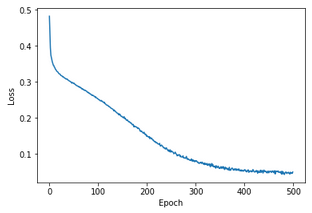
\includegraphics[scale=0.6]{Figures/chapter04/feature_engineering}
	\decoRule
	\caption[??]{??}
	\label{fig:FeatureEngineering}
\end{figure}

\\
\begin{figure}[h]
	\centering
	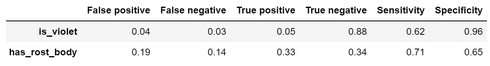
\includegraphics[scale=0.6]{Figures/chapter04/fe_table}
	\decoRule
	\caption[??]{??}
	\label{fig:FeatureEngineeringTable}
\end{figure}

\\
\textbf{Curvature prediction based on partial angles} \\
Although the accuracies are far from perfect the results appear to be promising. The hit rate for curvature detection is high: 82\% of all bended pieces were identified as such. In comparison, this holds for 71\% of the pieces affected by rust and 62\% of the violet pieces. In contrast, almost all pieces that are identified not to be violet are labeled accordingly (96\% specificity) whereas the specificity for rust (65\%) and curvature (67\%) is lower. The receiver operating characteristic reveals that the prediction is of better quality for violet and curvature prediction as compared to rust prediction which is reflected in a smaller area under the curve. Possibly this reflects that rather small brown spots were considered rust by some coders. \\

\begin{figure}[h]
	\centering
	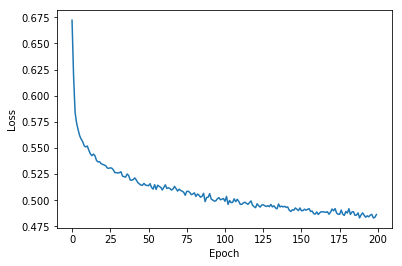
\includegraphics[scale=0.6]{Figures/chapter04/fe_curve}
	\decoRule
	\caption[??]{??}
	\label{fig:FeatureEngineeringCurve}
\end{figure}
\\
\begin{figure}[h]
	\centering
	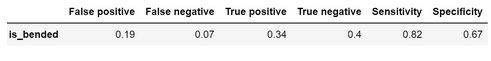
\includegraphics[scale=0.6]{Figures/chapter04/fe_curve_table}
	\decoRule
	\caption[??]{??}
	\label{fig:FeatureEngineeringCurveTable}
\end{figure}
\\
Considering the low agreement in labeling, higher values for the specificity and sensitivity of the classifier were not expected. A likely explanation is that the model generalizes deviating understandings and incongruencies we had when attributing labels and affected the reliability of the data. Arguably only little information was discarded by computing the sparse representations that served as an input. Information about irregularities in the outline that a center line does not reflect but possibly contribute to the perception of curvature and the spatial distribution of colored pixels might contain additional information regarding rust and violet-detection. However, the major criteria are captured. As MLPs have little hyperparameters that are suitable for non-linear mappings and  as the task of mapping high level features to human estimates appears to be rather simple, one could argue that there is little potential to improve the predictive quality using other techniques. By introducing a bias, the sensitivity (true positive rate) of the classifier can be adjusted at the cost of more false positives. Introducing a bias means that the threshold that is used to convert the floating point outputs of a neural network to booleans that indicate whether a feature is present or not can be set to values other than 0.5. The possibility of making the classifier more or less sensitive appears to be a good option to be implemented as a feature for customization by the user in asparagus sorting machines. The resulting behavior is reflected in the receiver operating characteristic that is calculated using different biases. \\
\\
\begin{figure}[h]
	\centering
	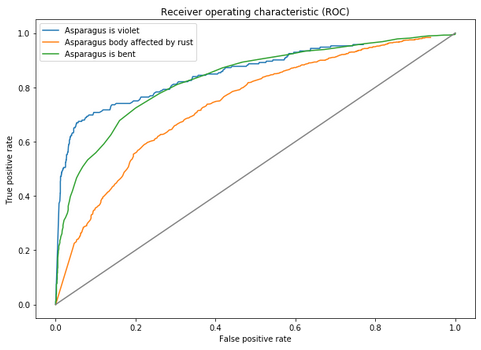
\includegraphics[scale=0.6]{Figures/chapter04/fe_roc}
	\decoRule
	\caption[??]{??}
	\label{fig:FeatureEngineeringROC}
\end{figure}

\subsubsection{A dedicated network for head-related features}

Some features relate to the asparagus heads only. Hence, it was assumed that classification is easiest when training a convolutional neural network on depictions of the respective region of the asparagus. Therefore, a dataset that consists only of images of the head area was used. Images of all three perspectives were appended horizontally such that each sample contains the information from all available viewpoints. This is especially important as rust affected spots are sometimes only visible from some angles. The depiction below shows one sample of rust affected asparagus heads. \\
\\
\begin{figure}[h]
	\centering
	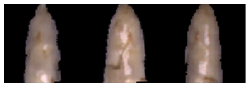
\includegraphics[scale=0.6]{Figures/chapter04/fe_head}
	\decoRule
	\caption[??]{??}
	\label{fig:FeatureEngineeringHead}
\end{figure}

A simple feedforward convolutional network was trained on the images. The features “flowering head” and “rust affected head” were chosen as target categories. The network comprises the input layer, ?? convolutional layers with kernel size ?? and ??, a fully connected layer with ?? neurons as well as the output layer. For the final layer the sigmoid activation function was applied while the hidden layers have RELU activations. A dropout layer was added to avoid overfitting. The network was trained using mean squared error (MSE) as an error function. The development of loss in the learning curve indicated convergence after 40 epochs. \\
\\
\begin{figure}[h]
	\centering
	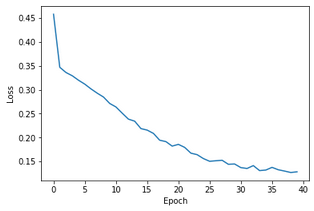
\includegraphics[scale=0.6]{Figures/chapter04/fe_head_curve}
	\decoRule
	\caption[??]{??}
	\label{fig:FeatureEngineeringHeadCurve}
\end{figure}
\\
The results for both features showed to be highly specific. In contrast the sensitivity is rather low. Only 55\% of the asparagus pieces labeled as “flowering head” were identified as such whereas the true positive rate is only 19\% for “rust head”. Given the low labeling agreement for these criteria these mediocre results are not surprising. \\
\\
\begin{figure}[h]
	\centering
	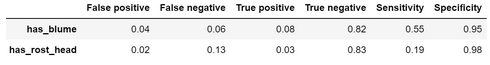
\includegraphics[scale=0.6]{Figures/chapter04/fe_head_table}
	\decoRule
	\caption[??]{??}
	\label{fig:FeatureEngineeringHeadTable}
\end{figure}
\\
The ROC curve indicates how the classifiers respond to the introduction of a bias and shows the overall prediction quality. The area under the curve is small for the feature “rost head”. Beside incongruencies in the labels this is possibly due the choice of the head region. It might be the case that brown spots in regions other than the cropped head were considered as an indicator for a rusty head when attributing labels. Improvements by increasing the cropped head region appear to be possible. \\
\\
\begin{figure}[h]
	\centering
	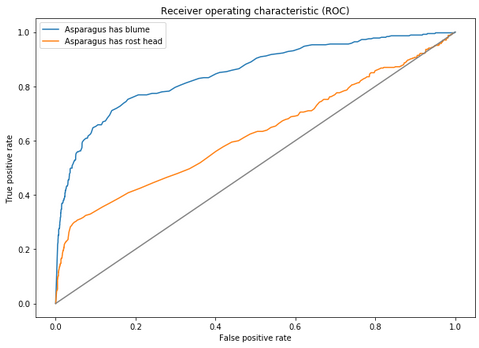
\includegraphics[scale=0.6]{Figures/chapter04/fe_head_roc}
	\decoRule
	\caption[??]{??}
	\label{fig:FeatureEngineeringHeadROC}
\end{figure}



\subsubsection{Single-label classification}

TODO

One supervised approach used for training a model on image data is a convolutional neural network (CNN). The approach was tested for our data with the application of a single-label classification CNN. A CNN uses trainable filtering kernels to extract features from an image and projects these features on feature maps (source XX). Based on these maps, the label is predicted by a standard multi-layer perceptron. \\
\\

BACKGROUND\\
→ TODO \\
\\
\\
STRUCTURE \\
The model architecture is roughly based on AlexNet but was strongly simplified to the level of variability and complexity of the underlying data. The network comprises four hidden layers: a convolutional layer, followed by a pooling layer, a second convolutional layer, and a dense layer. The input is an array of multiple horizontally stacked images. This input is trained on a set of binary labels containing information on whether the respective feature applies to the current image. The output of the network gives a prediction on each entered image gated by a sigmoid function on a range between 0 and 1. The rounded integer values of this output give a prediction of the apparent label. For the training of the model, the Adam optimizer was used because of its general acceptance as the state of the art optimizer for backpropagation (source XX). As a loss function binary crossentropy was used as it promised good results for single-label classification tasks (source XX). \\
\\
When training artificial neural networks, it can be difficult to find clear guidelines on how to implement an architecture such that an optimal training performance is given.
Hence, the idea was to start with the simplest form of a CNN and then gradually increase the complexity of the net. While AlexNet provides a good baseline for an image classification network, its architecture is still unnecessarily complex for the given task (source XX). The architecture was reduced to the minimum number of layers and parameters needed for a CNN. Over the period of training optimization, various processing steps and hyper-parameters were implemented and compared according to their performance. During this process, the data was split between training and validation data in order to have a reasonable overview on the possible test performance and to prevent direct overfitting.
The course of the hyper-parameters is explained in the following. \\
\\
Batch size \\
The batch size was initiated comparatively low with 64 samples per batch but soon increased to a value of 512 samples per batch. The large batch size was implemented in order to guarantee the convergence of the training data, since smaller batch sizes resulted in jumping gradients which were not able to converge into any minimum (source XX). \\
 \\
Learning rate \\
Various learning rates were tested during the optimization process. The initial learning rate of 0.003 (which is the standard learning rate for Adam optimizers in tensorflow (source XX)) was soon found to be too large to guarantee convergence of the algorithm. Thus, the learning rate was gradually decreased and found to be most effective in the range of 0.000001 (= 1e-6) to 0.00000001 (= 1e-8). Learning rates as small as 0.00001 (= 1e-5) still seemed too large for training the net. In addition, a gradually decreasing learning rate was implemented in order to make the training more effective (source XX).
 \\
Layer/Deepness \\
Starting with the smallest layer size possible, more layers were added based on the amount of theoretical background (source XX), which includes filtering steps … For example, for the feature fractured one layer for edge detection should have sufficed or for the feature violet a layer for colour detection. For other features, such as bent, at least two convolutional layers were expected to be more helpful (source XX). During the training process, it was settled to a model with two convolutional layers, one max pooling layer and one hidden dense layer. \\
 \\
Layer width/Number of kernels \\
A small number of kernels was thought to be enough compared to the kernel size of AlexNet (why? source XX). The kernel size resulted in 32 5x5 kernels for the first convolutional layer and 64 3x3 kernels for the second convolutional layer. These sizes were assumed to be sufficient, especially since increasing the number of kernels did not lead to any better results. \\
 \\
Exploding gradients /  Batch normalization \\
Both convolutional layers were built with batch normalization nearly from the start of implementation of the network. To guarantee that exploding gradients posed no problem, the gradients were inspected visually and the results gave no reason for assuming prolems with exploding gradients. \\
 \\
Epochs / steps \\
In most cases, 300 training steps were performed for the training. \\
 \\
Balancing the train data \\
A next step was to weight the loss function because of the largely unbalanced data. This ended with no better results, however, as the model still tended to make an unbalanced prediction by classifying all values as 0.0. Another idea was to reduce the dataset to make the number of images with the regarding feature even to the number of images where it is not present. This translates to throwing away valuable data, which can otherwise provide information about negative cases to support the model in it’s training. Thus, it was decided to keep all data images and instead balance the data by multiplying the minority of samples to match the number of negative samples. As there was no feature positively exceeding a presence of 50\% in the data, only positive labels were multiplied. \\
\\
Data augmentation \\
To improve training performance, some kinds of data augmentation were implemented. First, the images were flipped horizontally. These seemed to be a valid enhancement to the training data since it resulted in similar images to the original data. Additionally, small changes in the image angle (up to 5°) were tested, however, this type of data augmentation was neither effective nor convenient to be computed on the grid since an additional library would have been necessary to install. \\
\\
\\
RESULTS \\
→ TODO \\
\\
\\
DISCUSSION \\
→ TODO \\



\subsubsection{Multi-label classification}


Building on the standard single-label classification we were further interested whether it would be possible to build a model that can predict several feature labels at the same time. A multi-label classification model hereby gets an image as the input and learns to predict the presence or absence of several classification objects, in our case the feature labels. \\
For our model we decided to use a small convolutional neural network as described below and the features that we labeled by hand. Each of the six classes (hollow, flower, rust head, rust body, bended and violet) is encoded by a binary output in the target vector, indicating whether the asparagus exhibits the feature in question or not. \\
\\
BACKGROUND \\
Multi-label classification is a useful tool that can be used in classification problems in which several classes can be assigned to a single input. In contrast to a multi-class classification, where the model is supposed to predict the most likely class for an input, the multi-label classification makes a prediction for each class separately, determining whether the class is present in the image or not. While the different classes are mutually-exclusive in the multi-class classification, they can be related in the multi-label classification. Further, there is no limit on how many classes can be depicted in one image. It is also possible that all or none of the classes are present. \\
One could think of the multi-label classification task as consisting of different sub-tasks. Therefore, some multi-label classification problems can be transformed. There are two eminent ways to do so, either the problems  are transformed into multiple binary classification tasks or into one multi-class classification task. \\
In the first approach, a new model for each feature is trained, which are then combined to give a single output. That means that all features are independent of one another, because they are learned separately. This can be seen as one of the major drawbacks as it is not always clear whether features are related or not and in many cases they are. \\
Therefore, we decided to not only use single-class classification as described in chapter 4.1.3 but to explore the possibilities of multi-label classification. \\
\\
In the second approach, each possible combination of features is interpreted as one class. For a classification problem with 6 features that means there are 64 classes to be learned. The problems with this approach are, on the one hand, the exponentially increasing number of classes, and on the other hand the sparsity of samples per class. In many cases, some of the classes will be highly underrepresented or even empty. For that reason we decided not to elaborate this approach further and implement a model for multi-label classification without transforming the task to a multi-class problem. \\
\\
Inspiration for the model gave a blogpost[1] which aims to classify images of the MNIST fashion dataset in the context of multi-label, rather than multi-class classification. The author altered the dataset in such a way that each input image contains four randomly selected items from the MNIST fashion dataset. The model then learns to predict which classes are present in the image. There is no restriction on the random selection, therefore the items can be all from the same class, from four different classes or anything in between. The target vector has 10 values, one for each class, which are either 0 or 1 depending on whether that class can be found in the input image or not. \\
\\
This model was chosen as inspiration for two main reasons. Firstly, it tackles a similar problem as ours. In both cases, the model is supposed to predict the presence or absence of different fashion items or labeled features, respectively, and the number of classes is similar, it is 10 in the fashion example and 6 for our model. \\
\\
Secondly, the model uses a dataset of similar size, 9000 images were used for training and 1000 for validation, while we were training on 10800 images and validating on 1200. Despite the rather small dataset in comparison to many other machine learning problems, good results with an accuracy of 95-96\% were reached. This leads us to think, it might be a model with a good complexity for our problem too, as it is complex enough to yield good results, but not too complex for the medium-sized dataset. \\
\\
MODEL STRUCTURE \\
A classical convolutional neural network was chosen for the multi-label classification task. It consists of five blocks of convolution layers with max pooling layers followed by a global average pooling layer and a dense layer. \\
\\
In contrast to multi-class classification models, where usually a softmax activation function is used in the last layer together with a categorical cross entropy loss, the multi-label classification model uses a sigmoid activation function and a binary cross entropy loss. \\
\\
As the input of the model a concatenation of the three perspectives of each asparagus piece were used in order to maximize the information the model gets about each asparagus. This yields input images that look like the three asparagus pieces are laying side by side. Further the images were downscaled by a factor of 6 to facilitate training.
The output, or target, of the model is a vector of length six in which each position encodes one of the six hand-labeled features (hollow, flower, rust head, rust body, bended and violet). Each feature can either be applicable to the input or not, which leads to a "1" or "0" in the target vector, respectively. \\
\\
Several loss functions were tested to improve the models performance. For example, the hamming loss, which uses the fraction of the wrong labels to the total number of labels. Additionally to the in-built loss functions from keras, a custom loss function was implemented, that penalizes falsely classifying ones as zeros more than falsely classifying zeros as ones. The motivation for this custom loss was the fact that the two labels "0" and "1" are highly unbalanced. As previously stated, there are noticeably more zeros than ones in many classes. Hence, the model can get a decent accuracy by labeling most features as zero. By penalizing this error more, we intended to counteract the unbalanced dataset. But at the end, the binary cross entropy loss remained the one with the best results. \\
Further, it was tested whether regularization would improve the performance of the model on the validation data by preventing overfitting. For this, the model was trained by adding L1 or L2 regularization, respectively, to all five of the convolutional layers.  Hereby, a kernel regularization was implemented with a value of 0.01. \\
\\
L1 and L2 regularization can both be interpreted as constraints to the optimization that have to be considered when minimizing the loss term. The main difference between the two is that L1 regularization reduces the coefficient of irrelevant features to zero, which means they are removed completely. Hence, L1 regularization allows for sparse models and can be seen as a selection mechanism for features. As the inputs to our model are images, that consist of a large number of pixels, and additionally a large portion of those pixels are black, because the background was removed, it appears to be a good idea to reduce the number of features taken into account in the early layers. L2 regularization, on the contrary, does not set coefficients to zero, but punishes large coefficients more than smaller ones. This way the error is better distributed over the whole vector. \\
\\
\begin{figure}[h]
	\centering
	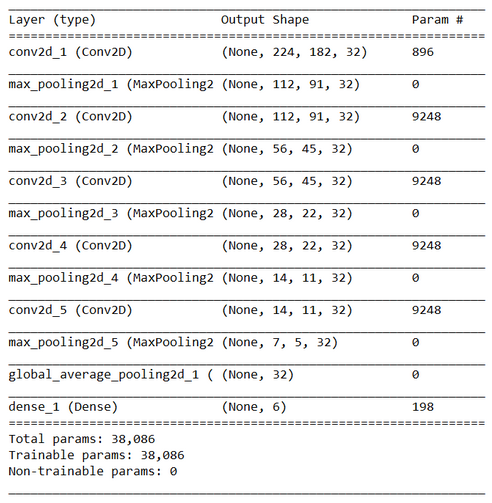
\includegraphics[scale=0.6]{Figures/chapter04/multilabel_structure}
	\decoRule
	\caption[??]{??}
	\label{fig:MultilabelStructure}
\end{figure}

RESULTS \\
As one can see in the figures XX-YY, all the different approaches explained above show a similar behaviour in accuracy and loss values. The training and validation accuracy increase slowly but steadily with the training accuracy always being a little higher than the validation accuracy. The training loss decreases rapidly, while the validation loss only decreases very little and shows random fluctuations. This can be an indicator for overfitting. Usually, L1 and L2 regularization are used to prevent overfitting, but in our case it did not improve the results, as one can see in figure XX. \\
When looking at the true positive rates, also called sensitivity, and the true negative rates or specificity, one can see that both increase during the training process , while the false negative and false positive rates decrease with the same slope. The false positive and false negative rates are mirror images to the true positive and true negative rates with the mirroring axis at the 50\% mark. It can be observed that the rates change rapidly in the first two to four epochs, after which the change progresses slowly in the same direction with no greater disturbances. One exception is the model trained with the L2 loss, which does not show a large change in either of the rates. \\
\\
\begin{figure}[h]
	\centering
	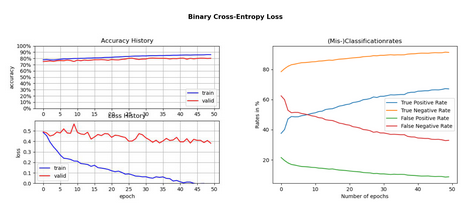
\includegraphics[scale=0.8]{Figures/chapter04/multi_crossent}
	\decoRule
	\caption[??]{??}
	\label{fig:MultilabelCrossentropy}
\end{figure}
\\
\begin{figure}[h]
	\centering
	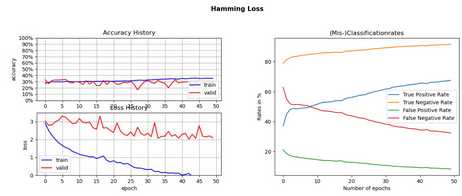
\includegraphics[scale=0.8]{Figures/chapter04/multi_ham}
	\decoRule
	\caption[??]{??}
	\label{fig:MultilabelHammingLoss}
\end{figure}
\\
\begin{figure}[h]
	\centering
	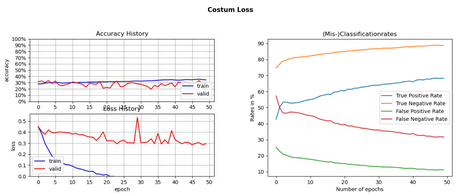
\includegraphics[scale=0.8]{Figures/chapter04/multi_costum}
	\decoRule
	\caption[??]{??}
	\label{fig:MultilabelCostumLoss}
\end{figure}
\\
When comparing the three different loss functions, it is noticeable that the binary cross entropy loss has significantly larger accuracy values than the hamming loss and the costum loss. Its values start at 75\%, while they start at around 30\% for the other two loss functions. The behaviour of the curves and the (mis-)classification rates, however, are very similar in all three approaches. The true negative rates start off very high with values around 80\% and increase further during the training. The true positive values start off lower, at around 40\% to 45\%, and increase rapidly in the first few epochs, after which the rates proceed to increase but with a narrower slope. As stated above, the false negative and false positive rates show the same slope but in the opposite direction.
\\
\\
\begin{figure}[h]
	\centering
	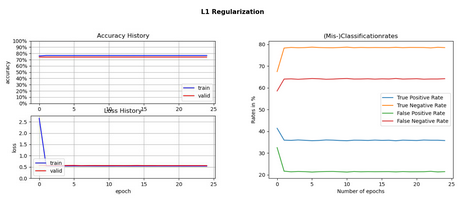
\includegraphics[scale=0.8]{Figures/chapter04/multi_reg1}
	\decoRule
	\caption[??]{??}
	\label{fig:MultilabelL1Regularization}
\end{figure}
\\
\begin{figure}[h]
	\centering
	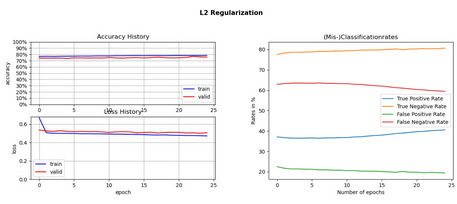
\includegraphics[scale=0.8]{Figures/chapter04/multi_reg2}
	\decoRule
	\caption[??]{??}
	\label{fig:MultilabelL2Regularization}
\end{figure}
\\
\\
The accuracy values of the models that were trained with L1 or L2 regularization, respectively, do not change over the epochs. The same holds for the validation loss. The training loss decreases in the first few epochs and remains stable after that.
While the (mis)-classification rates of the model trained with L1 regularization behave similarly to the ones trained with no regularization, the rates of the model trained with L2 regularization show a smaller increase and lack the fast change in the first epochs. \\
\\
DISCUSSION \\
The slopes of all curves indicate that the model is learning, because they are increasing in the case of the accuracy, sensitivity and specificity and decreasing in the case of the loss, false positive and false negative rates until the end of training. Hence, one might think that a longer training period will lead to better results. But the training loss decreases very rapidly while the validation loss does not. This suggests overfitting of the model, a problem which gets worse when increasing the training steps. Therefore, a longer training period most likely will not increase performance unless overfitting is prevented. As one can see in the result section neither L1 nor L2 regularization alone were able to prevent overfitting. Another common practice that could be tested is the drop-out, in which a certain amount of nodes are left out in different backpropagation steps. This way the model learns to not rely on a small number of nodes but distribute the information between all nodes available. Hence, the coefficients remain smaller. Another way to prevent overfitting is to reduce the model's complexity. A model with fewer parameters to train, is less prone to overfitting. A fitting degree of complexity should be found to model the data sufficiently good without losing the possibility of generalization. \\
\\
Accuracy alone might not be a good indicator to evaluate a multi-label model (QUELLE). As it highly depends on the loss function, it may have misleading results. This can be seen in the comparison between the three different loss functions. Although the sensitivity and specificity show similar values, the accuracy values suggest that the binary cross entropy loss outperforms the other two loss functions by far. The accuracy of the model trained with the binary cross entropy loss has an accuracy more than twice as high, but when looking at the slope of the curve it appears that the model with the binary cross entropy loss does not, in fact, perform better than the other two models, because all three have an increase of accuracy of roughly 10\% and a similar sensitivity and specificity. This indicates that the slope of the accuracy function can be considered to evaluate the training process of the model, but the real values should be interpreted with caution. \\
\\
One thing that comes to attention when looking at the (mis-)classification rates is that the true positive rates are a lot lower than the true negative rates. A reason for that might be that there are fewer positive values in the dataset and they are, thereby, more difficult to learn. The model might have learned that, if unsure, a zero is the more likely guess. \\
\\
The L1 and L2 regularization both seem to prevent the model from learning all together instead of only preventing overfitting. A reason for that might be that the regularization factor was too high. More experiments should be conducted with varying values to test this hypothesis. \\
\\
In summary, the model improves its sensitivity and specificity, but it seems like it does so by overfitting the training data. Therefore, the next step should be to prevent the model from overfitting and after this problem is solved, it should be tested whether additional changes can improve the performance of the model further. \\

\subsubsection{From feature to label}

Additionally to the feature classification tasks, we used supervised learning to predict the 13 commercial asparagus classes from the labelled features. As described in chapter XX we decided to label features rather than classes, therefore all the approaches described also learned to predict those features from the input images. To get to the final classes from the features is only a small step in theory and if we would be able to solve the problem of the feature classification task perfectly, the distribution in the commercial classes should not be problematic. Nonetheless, it is interesting to see how easily this translation can be done and especially how well the categories match with the ground truth that we established at the asparagus farm. \\
\\
In order to build a ground truth, we collected images of the 13 classes of asparagus that were ready to be sold as the specific class. That means, the asparagus was not only sorted by the machine but resorted by the experienced staff at the asparagus farm and the images were collected by running those re-sorted spears through the machine a second time. We then labelled these images with the label app and the labelled features were used as the input for the following supervised learning approach, while the known classes were used as the output or target. Approximately 200 images per category were used. \\
\\
Two different approaches were implemented and tested to predict the classes from the features. The first one is a simple model with X fully connected layers.\\
TODO: Model structure beschreiben\\
\\
The second approach is a random forest, with X number of trees, X number of features per branch and a depth of X for  each tree.\\
TODO: details/structure beschreiben\\
\\
Random forests are a popular machine learning approach, because they reach good results in both regression and classification tasks. Further, they are based on decision trees, which are frequently used because of their intuitive interpretation for humans. Although decision trees themselves are powerful tools, they have the major drawback of being prone to overfitting. Random forests aim to avoid this problem, while still using the advantages of decision trees, namely that they are flexible, easy to use and fast to train. They do so by training several decision trees on different random parts of the data, after which a majority voting decides on the final output or class. An additional trick that can be used is a random selection of features to be used at each branch. This reduces the influence of highly correlated features and thereby makes the random forest more robust.\\
\\
With this second approach, a score of 0.76 was reached, which is already very high compared to what the accuracy of 0.08 by random chance guessing would be. One way to increase the accuracy even further would be to increase the agreement on the labelled features. By reducing the amount of noise generated by ambigues labelling the performance might be enhanced. \\
\\
When comparing the results of the two approaches one can see...
\begin{itemize}
\item unified interface (labels + classes, scikit-learn & keras model compatibility)
\item metrics: look at classification report in streamlit multiple\textunderscore models app
\item simple keras model with fully connected layers etc., reaches an evaluation of 2.2
\item confusion matrices for both as figures, compare the different results
\item app: dataframe, diagrams, able to see the images and corresponding hand-labeled features and predicted categories
\end{itemize}

QUELLE~\citep{friedman2001elements}


\subsection{Unsupervised learning}

Unsupervised learning are all kinds of machine learning algorithms which are not supervised. More specifically, they work without a known goal, a reward system or prior training, and find a structure within the data, or some form of clustering of data points. In supervised approaches, the model is given both the input and the labels. In unsupervised learning approaches, the model is only given the input data. What this means is that unsupervised learning works without training samples, and without labeled data. One goal of unsupervised learning algorithms is tao find hidden structures or patterns in the data, without a given label. \\
\\
Dimension reduction algorithms and clustering algorithms have been identified as the two main classes of unsupervised machine learning algorithms which are used in unsupervised image categorization~\citep{article}. \\
\\
Multivariate datasets are generally also high dimensional. However, it is common that some parts of that variable space are more filled with data points than others. Large parts of high dimensional variable space are not used. In order to recognize a structure or pattern in the data, it is often necessary to reduce the number of dimensions. For this, both linear- as well as non-linear approaches can be applied. Linear unsupervised learning methods for which also descriptive statistics can be acquired are e.g. Principal Component Analysis (PCA), Non-negative matrix factorization, and Independent component analysis~\citep{article}. Some examples for non-linear approaches would be Kernel PCA,  ( Scholkopf  et  al. – im oben genannten paper),  Isometric  Feature  Mapping  (ISOMAP),  Local  Linear  Embedding,  and Local  Multi-Dimensional  Scaling  (Local  MDS). 
For the current work, the linear dimension reduction algorithm PCA was chosen.

\subsubsection{Principal Component Analysis}

PCA was chosen, because it is one of the standard methods of unsupervised learning in machine learning, to analyze data. Moreover, it is a linear, non-parametric method and widespread application to extract relevant info from high dimensional datasets. The hope is to reduce the complexity of the data, by only a minor loss of information (Shlens - A tutorial on PCA). Besides being a dimension reduction algorithm, PCA can also be useful to visualize the data, filter noise, extract features, or compress data. \\
\\
Our initial aim was to reduce the dimension of our dataset for further models. However, as this was performed at the beginning of the data inspection, we also had the aim to visualize our data in a three-dimensional space, in order to get a better understanding of the data distribution. The images that comprise our original dataset have a high quality, and instead of only reducing the pixel size, we aimed for reducing the information contained in named depictions by analyzing the principal components in a first step and projecting all relevant images into the lower dimensional space. This information could serve as the input for later machine learning algorithms in a second one. As we decided to use an approach for semi supervised learning that is based on neural networks later we focussed on the question what principal components reveal about the data. \\
 \\
PCA relies on linear algebra. It assumes that large variances are accompanied by important structure. When calculating the covariance matrix of the data, it reveals information about the overall structure and orientation of the data points in the multivariate space. The axis with the largest variance is set as the first principal component. It further assumes that the principal components are orthogonal to each other. Therefore, the second principal component is the highest variability of all directions which are orthogonal to the first one (Bohling  - Dim. Reduction and Cluster Analysis paper p.2). The covariance between each pair of principal components is zero, as they are uncorrelated. Generally, the higher the eigenvalues, the more useful it is for the analysis. \\
\\
The result of a PCA is a representation of the data in a new lower coordinate system, which depends on the axes of the largest variance. The dimensionality of this lower coordinate system should depend on the size of the eigenvalues. When plotting the data along the axes of the principal components, it is often easier to understand and interpret the data, than in the original variable space. \\
\\
It is a consensus in the literature, that PCA can be a good method to apply dimension reduction on images~\citep{turk1991face}~\citep{lata2009}.
However, there are several different ways on how to do so. First of all, it has to be decided if the PCA should be performed on a black and white image, or if a more complex approach on colorized images is needed. When working on black-and-white images, only one data point per pixel is given, therefore, performing a PCA is less computationally expensive, and also finding structure is easier. However, as we need to be able to recognize violet as well as rust, it was important to us, to be able to differentiate between color nuances, which cannot be represented in a black and white image. \\
 \\
There are at least three different ways on how to perform a PCA. First, it can be performed on images of different classes at the same time – similar as to capture several images of several people in one database, on which a PCA is performed. In our case this would mean that a PCA is applied to a dataset of several input images of all 13 classes of asparagus images. Second way would be to perform a PCA separately on each group. This way, an “Eigenasparagus” of each group would be calculated, and distances between Eigenasparagus of different groups could be measured. Third PCA can be employed feature-wise. In this case, the dataset would consist of a collection of images with a certain feature present vs a collection of the same size with the feature absent. \\
 \\
We calculated the PCA for black-and-white images, as well as on images without background, and also tried to work on all groups at the same time, group-wise as well as feature-wise. We decided to perform our final PCA on sliced RGB images with background, that are labeled with features by us with the hand-label-app, as this seems to yield the best results. An amount of 400 pictures per feature was considered to later on perform a binary PCA for each feature (either the feature is absent or present). \\
The 200 pictures where the certain feature is present as well as the 200 pictures where the certain feature is absent are extracted through a function in code/pca\textunderscore code/feature\textunderscore ids.py. This function loops over the combinded\textunderscore new.csv csv-file, where all hand-labelled information is stored as well as the path to the labeled pictures. For each feature a matrix is created, storing 200 pictures with the present feature and 200 pictures without the feature. E.g., m\textunderscore hollow is the matrix created for the feature hollow (shape = 400, img\textunderscore shape[0]$3\times4$ img\textunderscore shape[1]$3\times4$ img\textunderscore shape[2]). The first 200 entries in the matrix are pictures of hollow asparagus, the last 200 pictures show asparagus, which is not hollow. These matrices were calculated for the features hollow, broken, flower, rusty head, rusty body, bent, violet, length and width. \\
\\
For all these features, a PCA is calculated by first standardizing the matrix pixelwise (dimensions: 1340$3\times4$ 346$3\times4$ 3), calculating the covariance matrix and then extracting the ordered eigenvalues. The principal components are calculated multiplying these eigenvectors with the standardized matrix. The highest 10 eigenvalues were plotted to visually decide where to set the threshold of how many principal components will be further included. The feature space, the principal components and the standardized matrices are saved to later perform a recognition function. \\
\\
The recognize function is a control function, which performs on unseen images and tries to predict if a feature is absent or present. This function is also performed feature-wise. It reads in a new picture of one asparagus, which is not part of the asparagus database, so not within the 400 images. Then, it searches for this picture the most similar asparagus in the feature matrices (which are 200 pictures with the feature, 200 pictures without). \\
In greater detail, the input picture is first centered by subtracting the mean asparagus and then the picture is projected into the corresponding feature-space. That means the picture is “translated” into the lower dimensional space, in order to compare it to the known 400 pictures. The comparison is made through calculating the distance between the single centered eigen asparagus and the 400 pictures in the feature space, by using the cdist function of the SciPy software. The smallest distance is considered as the most similar asparagus. If the index of the most similar asparagus is smaller than 200 we know that the feature is present, if it is above the feature is absent. By comparing this to the information of the single asparagus piece, we know if the new asparagus has the same feature as its closest asparagus in the feature space, or not. By doing this for several images, we can already presume if the two features are likely to be easily separable or not. By evaluating this, we have a measure of how well our used principal components capture the distinguishing information of each feature. \\
\\
All preparation, calculation and analysis for the final PCA was performed in python (version x). All scripts ran in the virtual environment dataSet. The main packages used were cv2, SciPy and Matplotlib. \\

\begin{figure}[h]
	\centering
	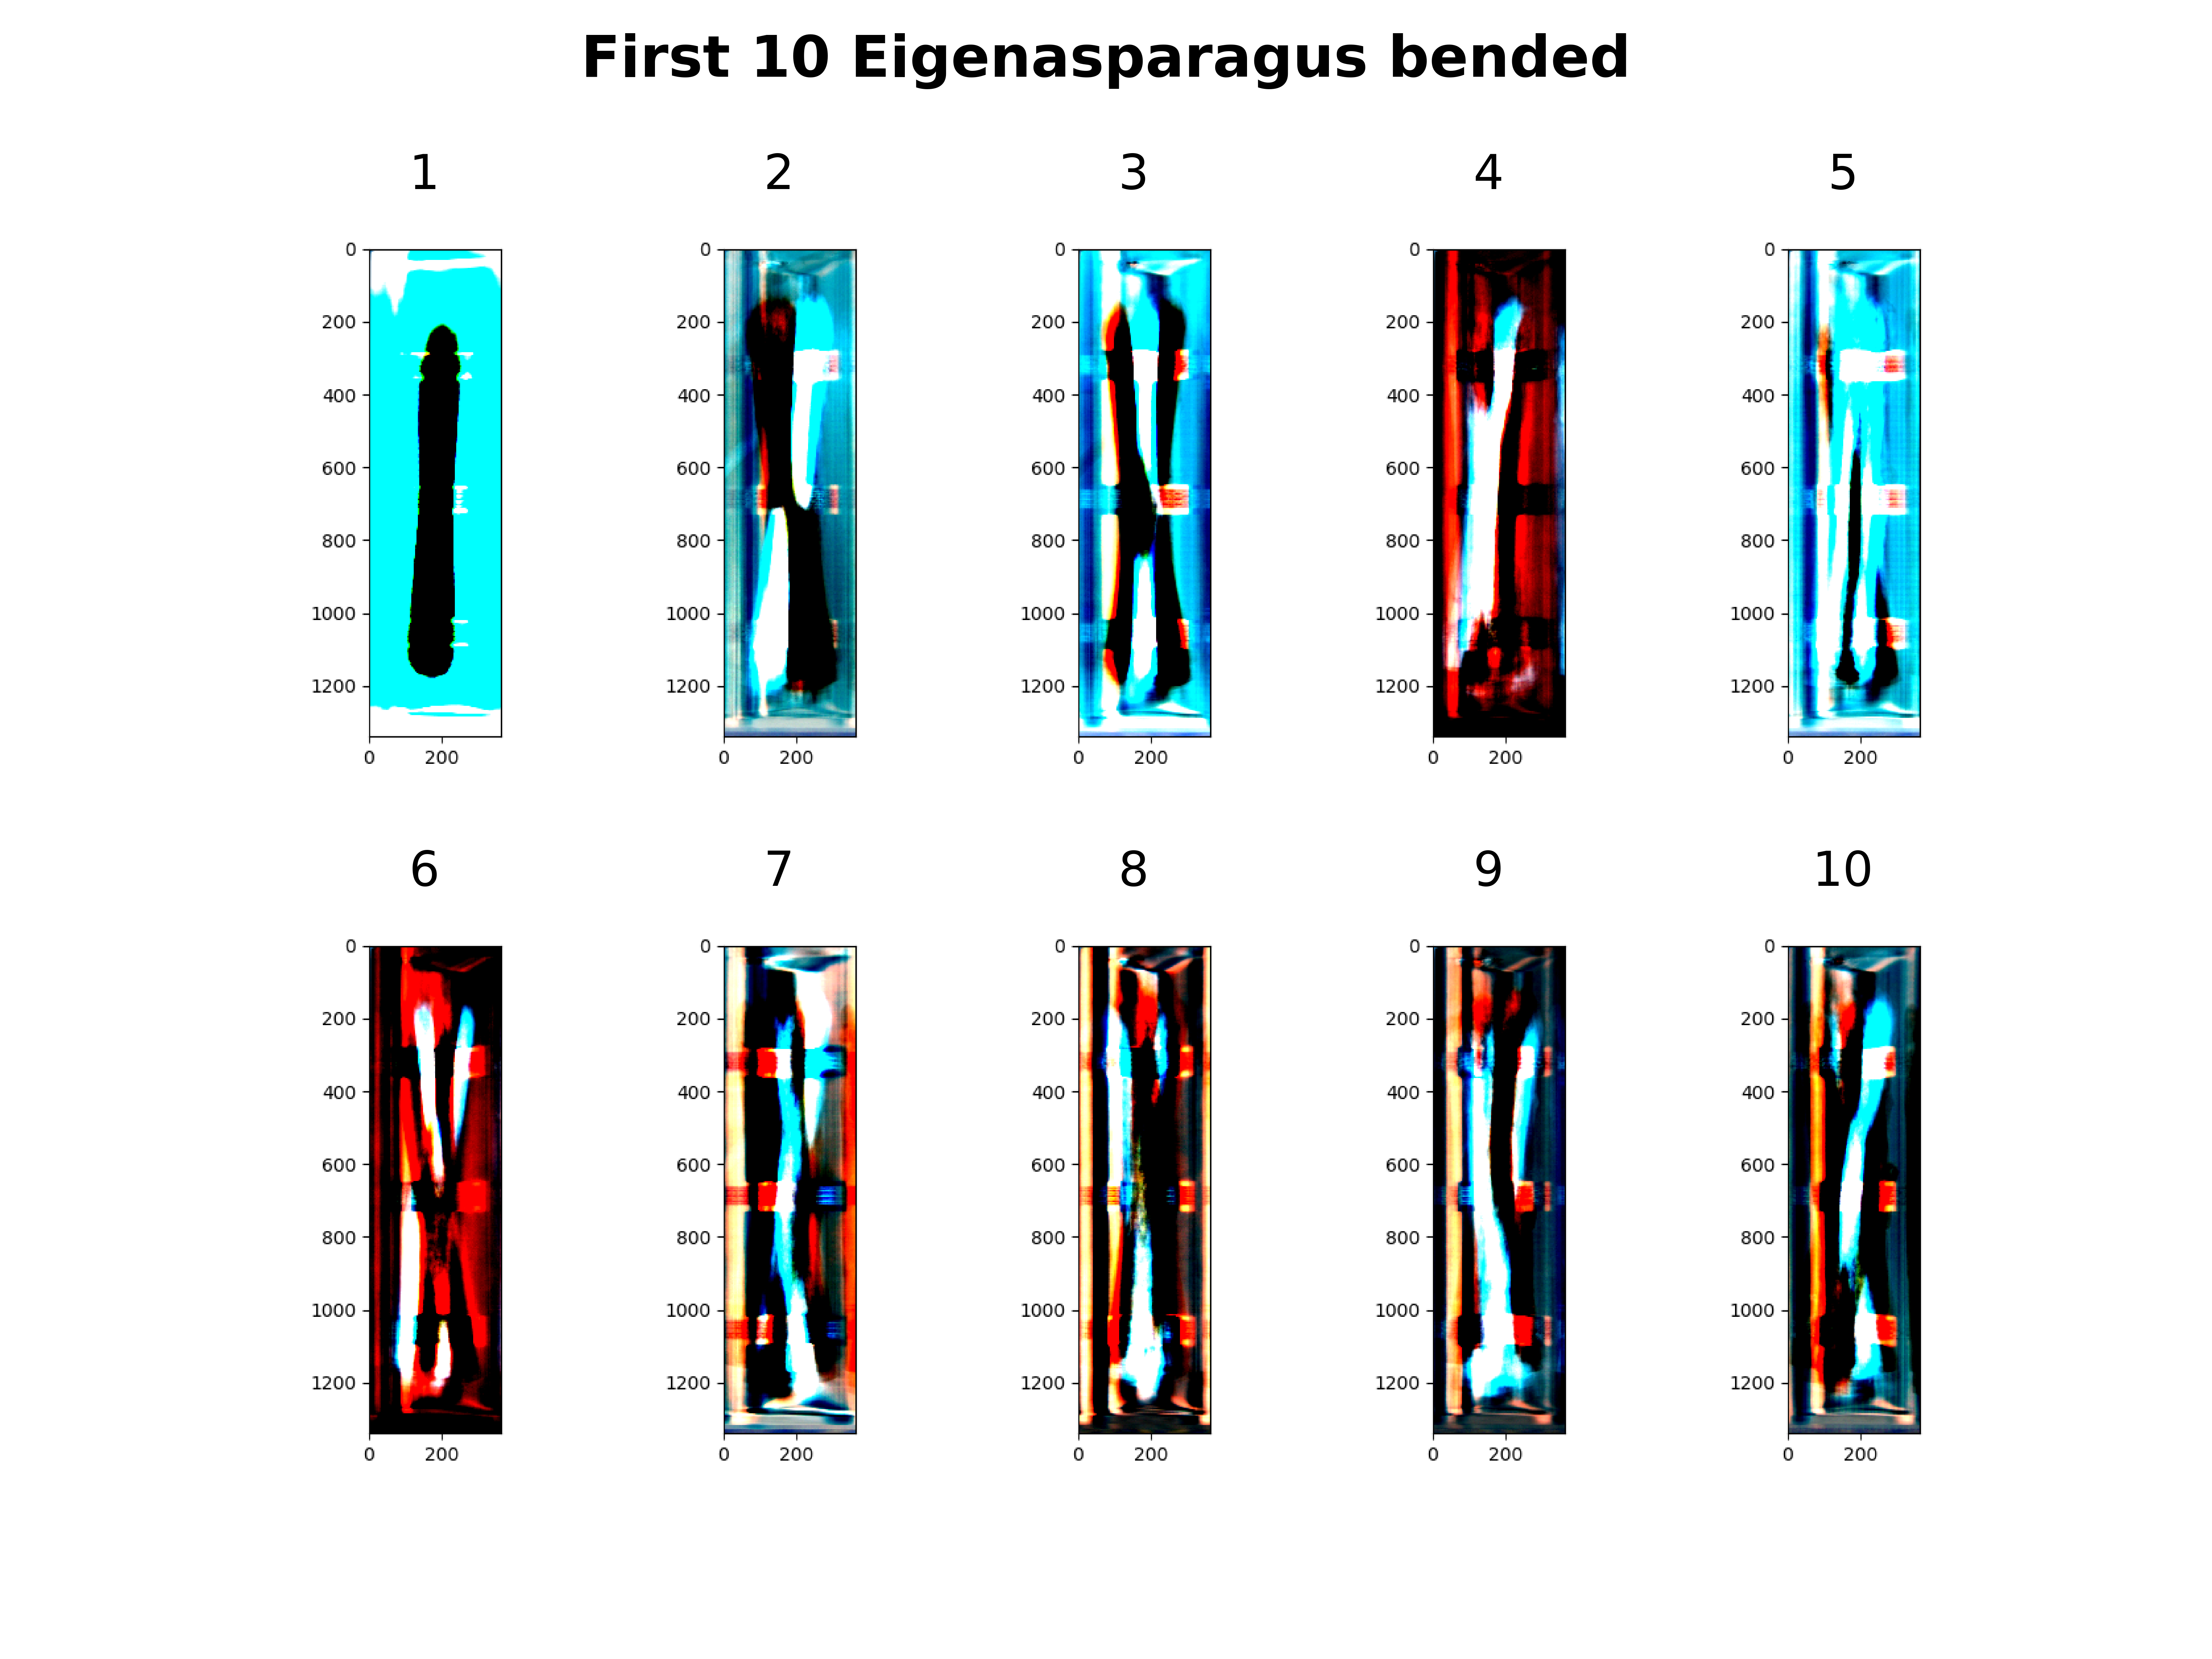
\includegraphics[scale=0.05]{Figures/chapter04/pc_bended}
	\decoRule
	\caption[??]{??}
	\label{fig:PrincipalComponentBended}
\bigbreak
	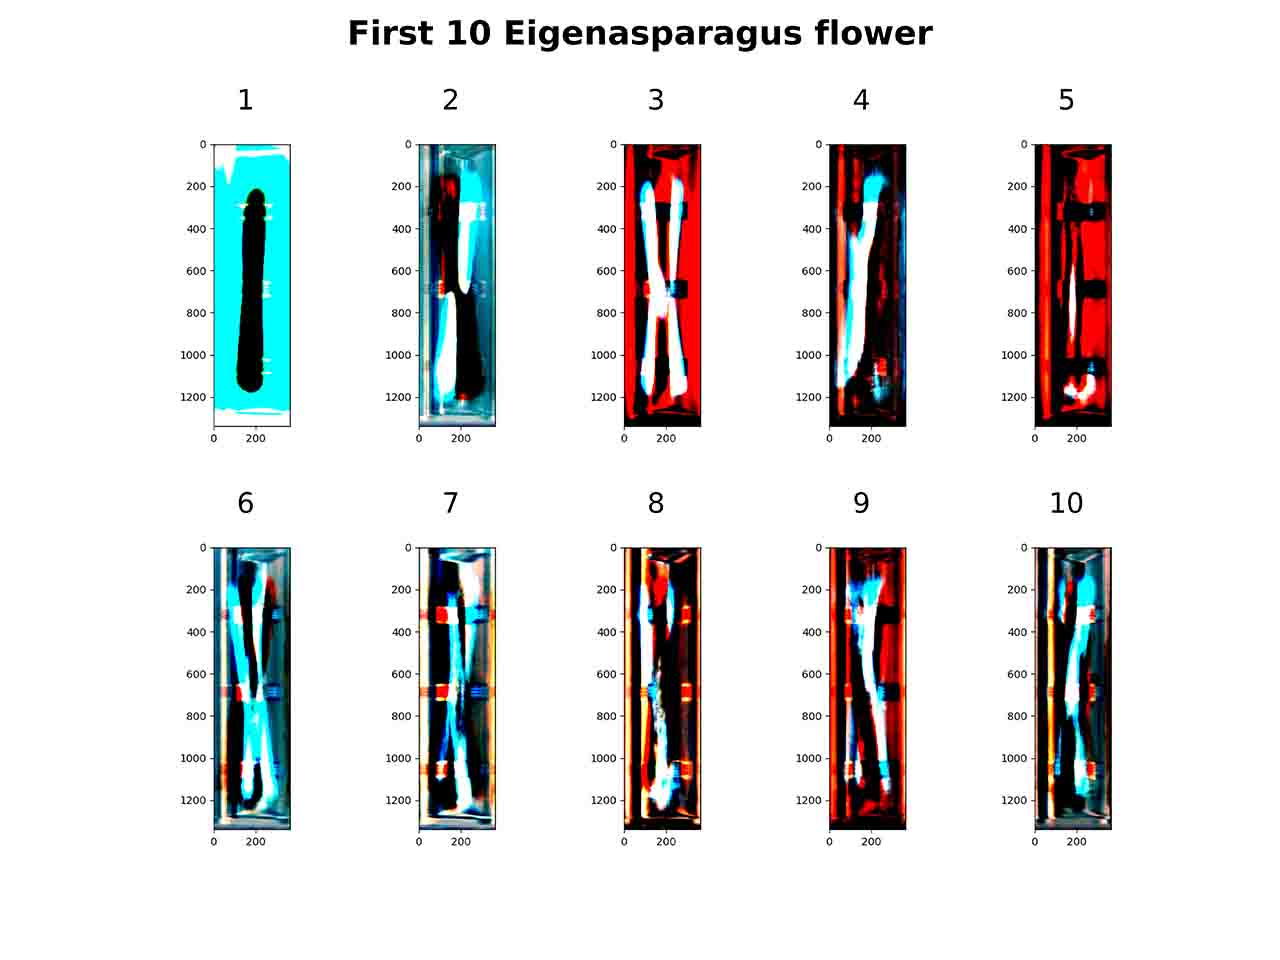
\includegraphics[scale=0.05]{Figures/chapter04/pc_blume}
	\decoRule
	\caption[??]{??}
	\label{fig:PrincipalComponentBlume}
\end{figure}
\\
The final results of our PCA are given feature-wise and were not translated back on the initial 13 groups. The features on which results are given are: hollow, flower, rusty body, bent, width and length. All features are binary. For the first five features, the manually hand-labeled information was taken, for the last two features, the information, which was extracted by the algorithms used in the hand-label app were taken. The decision boundary for the first five therefore depends on our predefined criteria on labeling. The decision boundary for width was narrower or equal to 20 mm or wider than 20 mm, for length shorter or equal to 210mm or longer than 210 mm. \\

\begin{figure}[h]
	\centering
	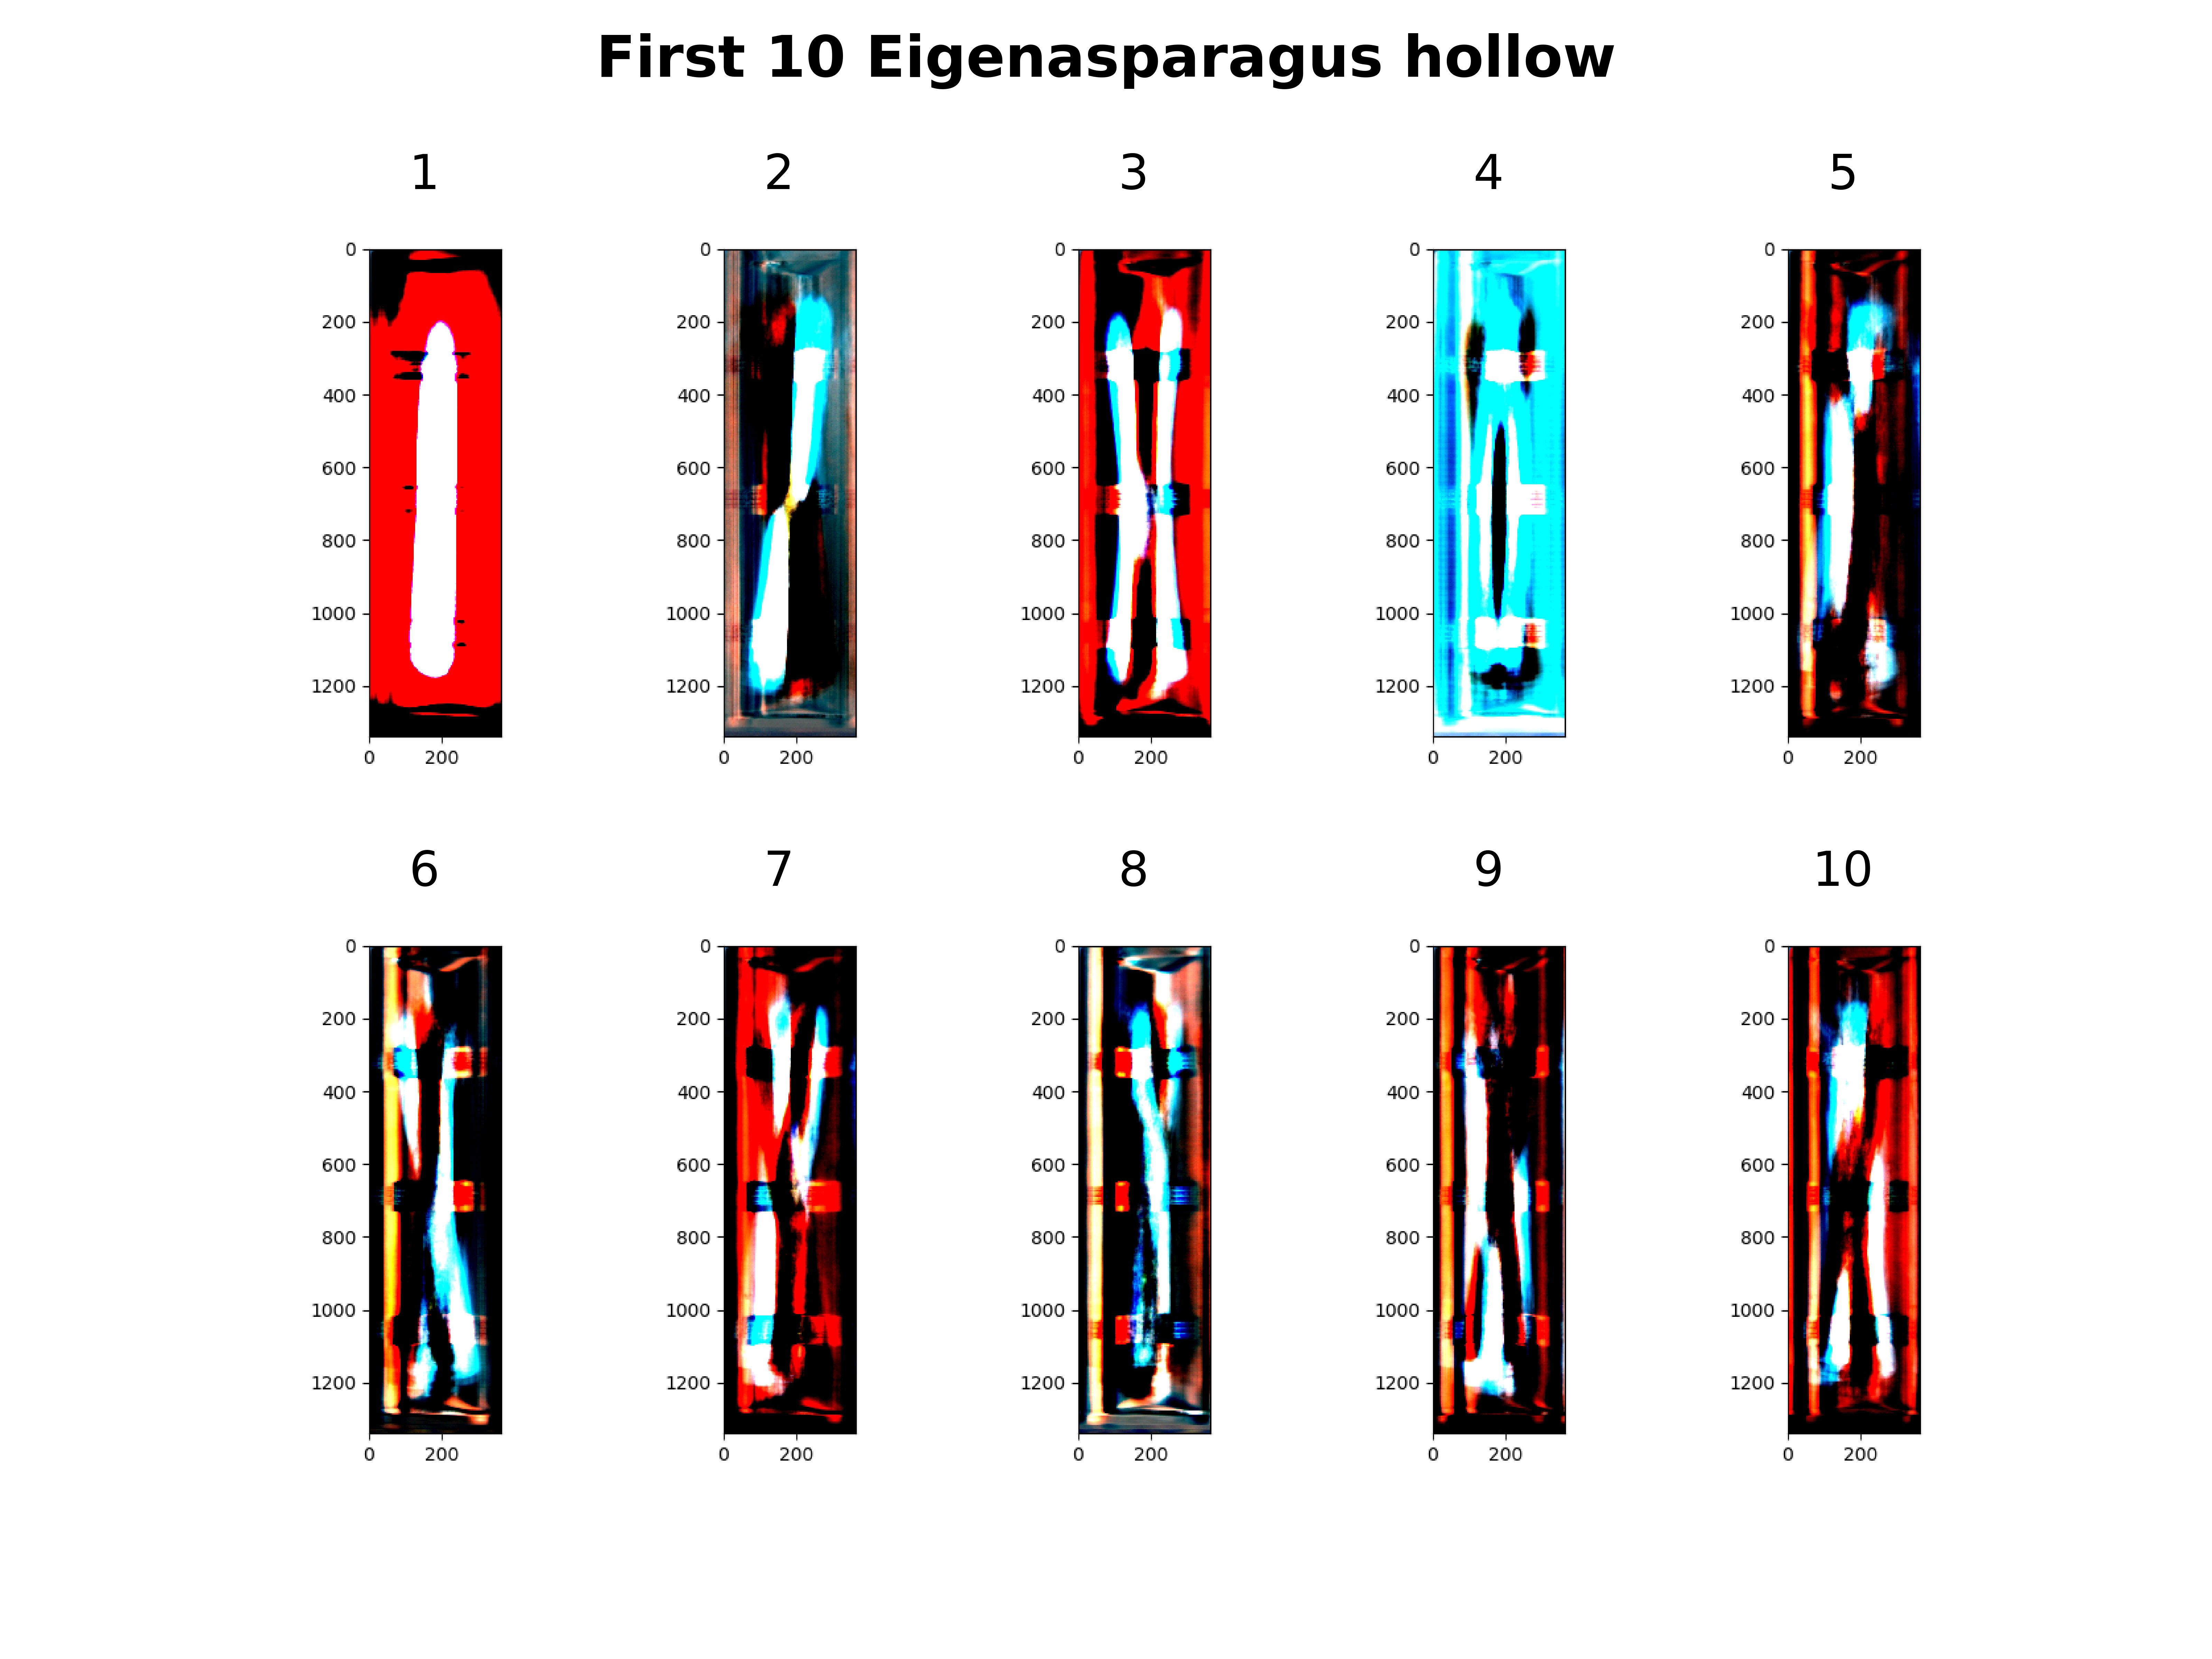
\includegraphics[scale=0.05]{Figures/chapter04/pc_hollow}
	\decoRule
	\caption[??]{??}
	\label{fig:PrincipalComponentHollow}
\bigbreak
	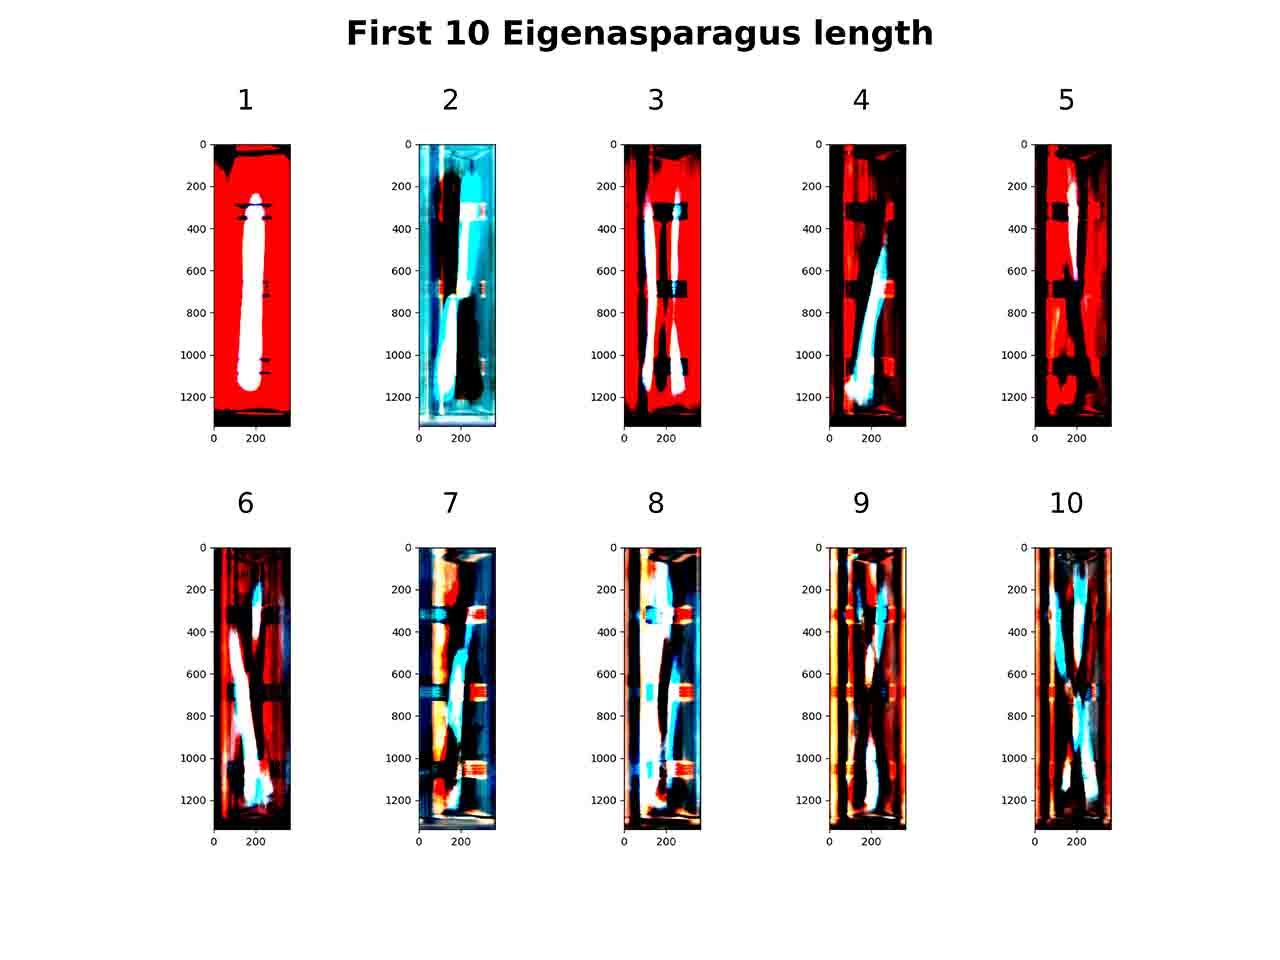
\includegraphics[scale=0.05]{Figures/chapter04/pc_length}
	\decoRule
	\caption[??]{??}
	\label{fig:PrincipalComponentLength}
\end{figure}
\\
There are no results for the feature broken, even though it is one of the initial main features, as there were only five labelled pictures for this category. Therefore, it was excluded for further analysis. \\
For the feature rust head, there was a problem in the calculation. For an unexplainable reason, there were complex values in the calculation of the principal components. Due to time constraints, this problem was not solved, yet. Therefore, plotting of the feature rust head was not possible. \\

\begin{figure}[h]
	\centering
	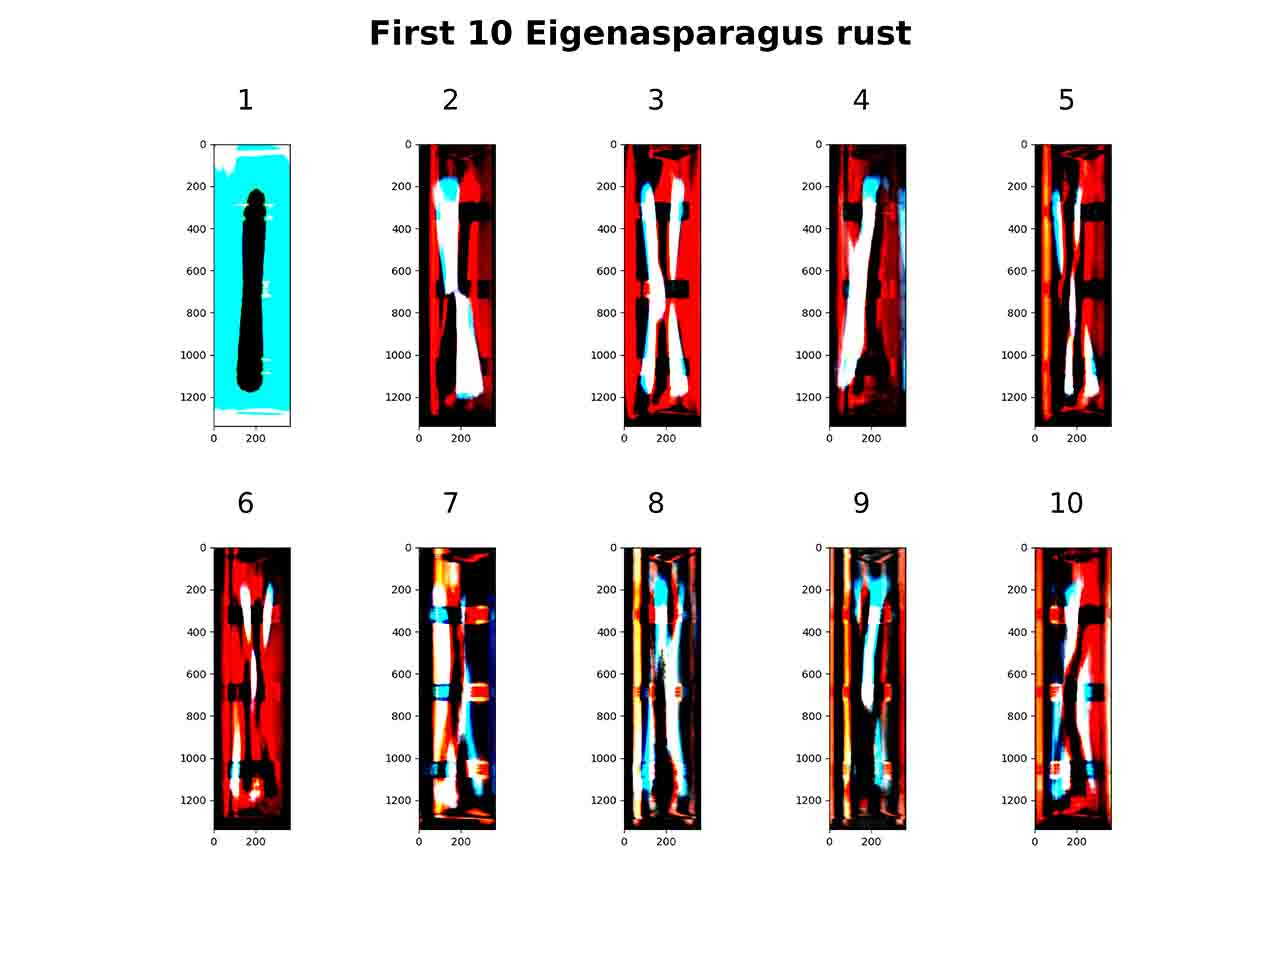
\includegraphics[scale=0.05]{Figures/chapter04/pc_rust}
	\decoRule
	\caption[??]{??}
	\label{fig:PrincipalComponentRust}
\bigbreak
	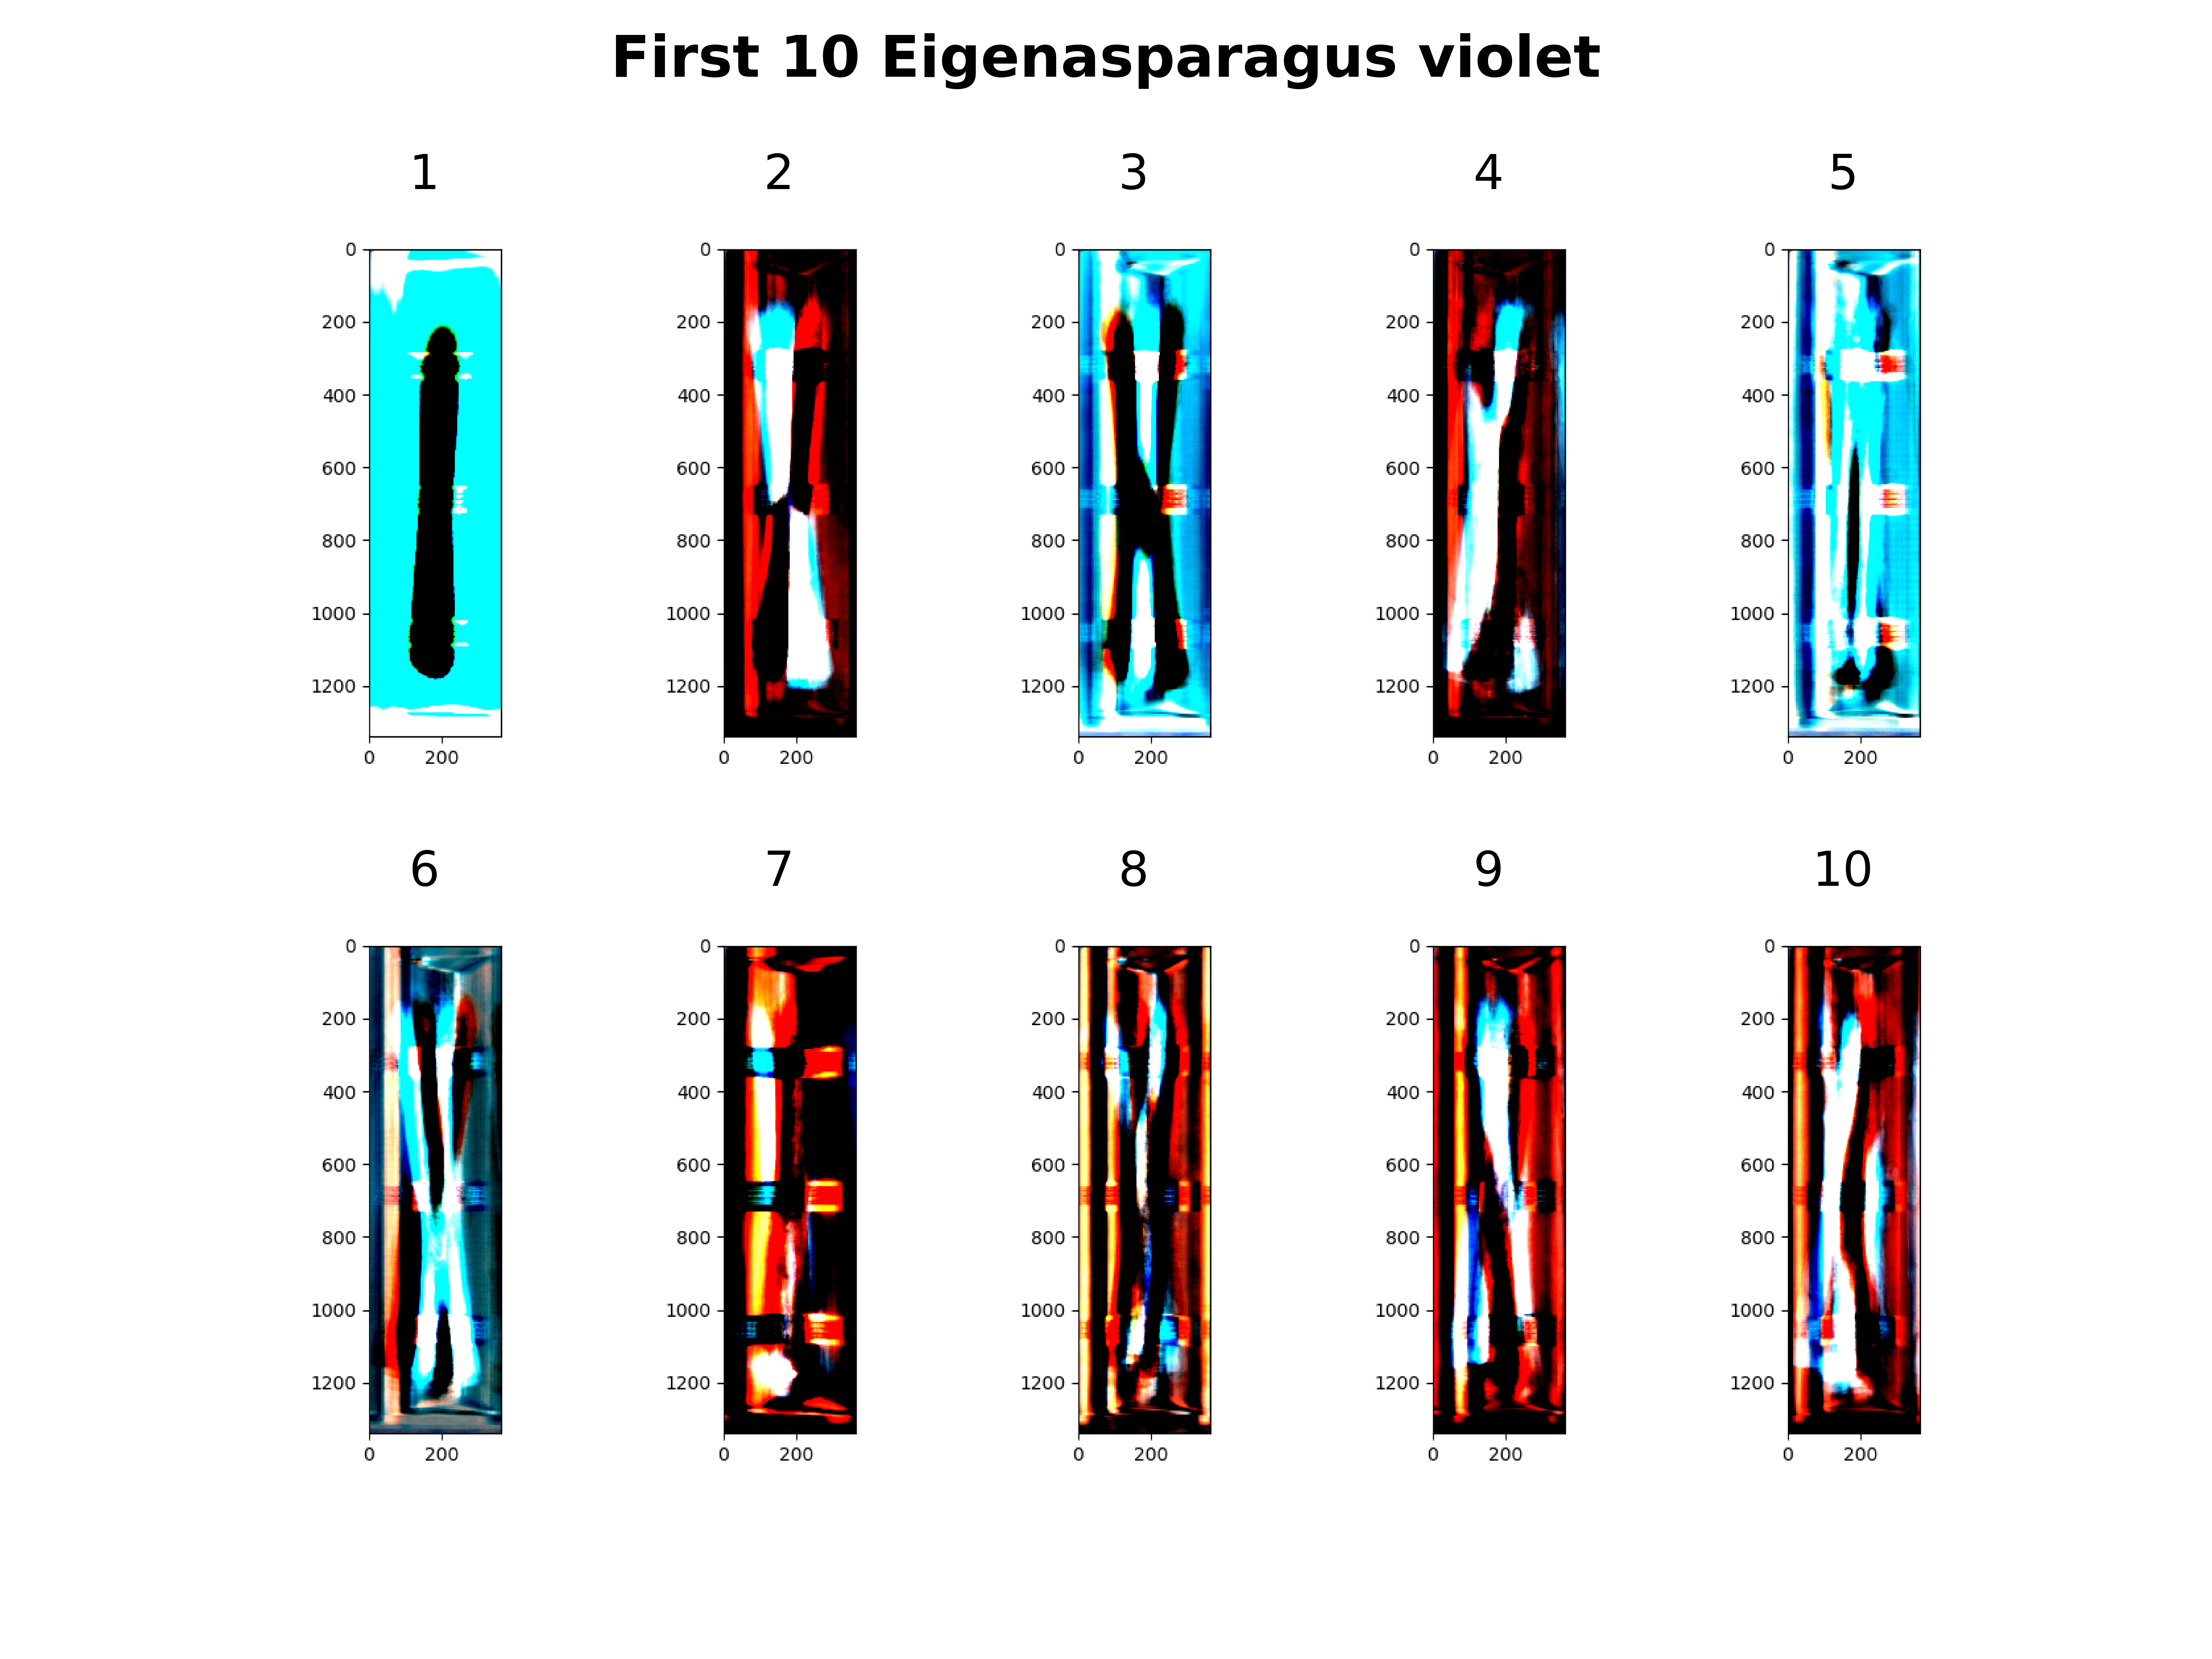
\includegraphics[scale=0.05]{Figures/chapter04/pc_violet}
	\decoRule
	\caption[??]{??}
	\label{fig:PrincipalComponentViolet}
\end{figure}
\\
By applying the feature\textunderscore pca.py file on each feature, the eigenvectors, eigenvalues, and principal components for each feature were computed and stored. In all cases, the first principal component is quite high (between X and X), and drops down rapidly afterwards. The values of the principal components after the 4th principal component are very low (below X). \\

\begin{figure}[h]
	\centering
	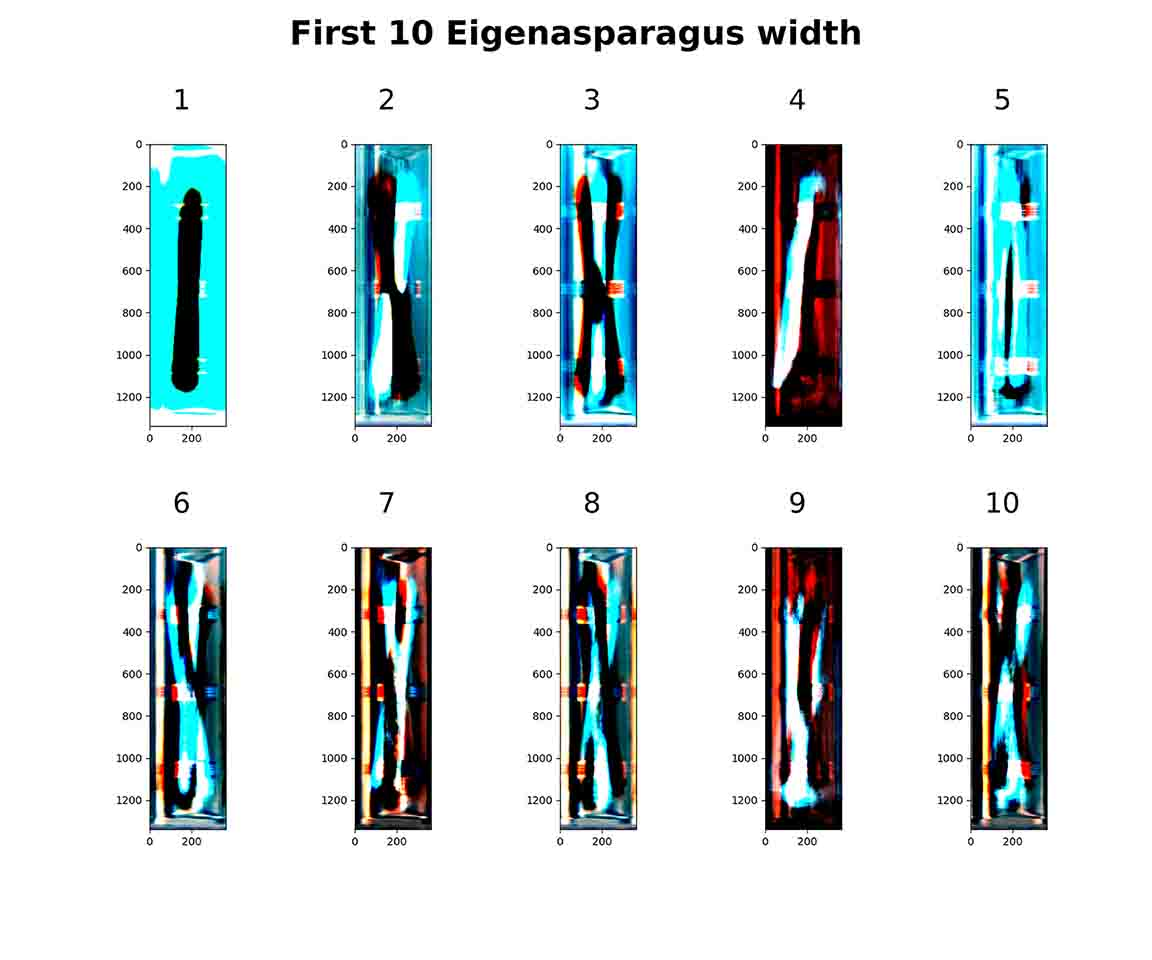
\includegraphics[scale=0.05]{Figures/chapter04/pc_width}
	\decoRule
	\caption[??]{??}
	\label{fig:PrincipalComponentWidth}
\end{figure}
\\
After inspection of the graph of the first 10 principal components, we decided that only the  first four principal components are used for the analysis, as there was either a sharp drop in the slope after the first 4 or to maintain continuity between the different features. Following, the corresponding feature space is that space spanned by the first four principal components. \\
 \\
We plotted the four-dimensional data in the feature space as scatterplots in three-dimensional space and the fourth dimension as color, but as it was difficult to interpret and visually understand, we decided to show plots of only the first two dimensions, here. 
\\ 
The following scatterplots show the data of each feature lined up along the axes of the first two principal components of each feature. \\

\begin{figure}[h]
	\centering
	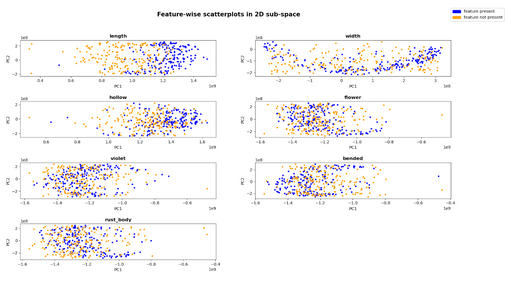
\includegraphics[scale=0.8]{Figures/chapter04/pc_2dspace}
	\decoRule
	\caption[Featurewise scatterplot in 2D]{Plotting the data in the 2D PC space for each feature.}
	\label{fig:PrincipalComponent2DSpace}
\end{figure}
\\
For the recognition function, we used the same 10 images, to test each feature. The classification worked best for the features length and hollow (10/10 classified correctly) and then width (8/10 classified correctly). It performed around chance-level for flower (6/10 classified correctly), violet and rusty-body (5/10 classified correctly) and extremely poor for bent (2/10 classified correctly).  \\
\\
 
DISCUSSION \\
The results we got for the final PCA approach, of calculating the principal components for each feature separately led to better results, then the first two approaches. \\
 \\
From the images of the first 10 principal components, we can visually assume that there is information about the length and shape stored in the first principal component, as a clear asparagus piece can be seen. The following images leave a lot of room for interpretation, about what information is contained there. \\
We performed the PCA on each feature separately, to extract the principal components of each feature. It is interesting to see that the pictures of the different features are all very similar. One reason for this might be that many of the 400 pictures for each feature are overlapping between features. Another reason might be, that even though the images vary between features, the general information of all asparagus images is very similar. \\
\\
From the results of the recognition function, one can see that there are large differences between the features on how well our PCA performs (20\% - 100\%). 
One reason for this could be that certain features are simply more difficult to distinguish than others. Another reason for this large variation can be that certain features are also more difficult to label consistently (see also chapter 3.4.3  (agreement measures)), and that the results are due to inconsistencies within the data. One indicator that this is a considerable reason is that the performance of the width and length features, which is information which is not hand-labeled, is very high. Moreover, the poorest results can be observed for the features bent and rust-body. Those are the features, for which the agreement measures showed the largest discrepancies between annotators (see 3.4.3). \\
 \\
Another reason why the results are partly only moderate, is that RGB image data possesses complicated structures, and by representing it in a linear low dimensional feature space, it might be that simply too much information is lost. Even though there are papers reporting good results on PCA on image data~\citep{turk1991face}~\citep{lata2009}, there are other papers claiming that nonlinear dimension reduction algorithms are needed for image data~\citep{article}. 


\subsubsection{Autoencoder}

Beside PCA, there are further techniques for dimensionality reduction. One alternative machine learning approach that can be employed to deduce sparse representations and automatically extract features by learning from examples are autoencoders. Simple autoencoders, where the decoder and encoder consist of multilayer perceptrons, were already proposed as an alternative to PCA in early days of artificial neural networks when computational resources were still comparatively limited~\citep{kramer1991nonlinear}.  Today one can choose from a multitude of network architectures and designs that all have one property in common: A bottleneck layer. For image classification it is common practice to use convolutional autoencoders. There are numerous papers that employed convolutional autoencoders in various domains. Examples range from medical images to areal radar images~\citep{chen2017deep}. These include not only shallow networks but more recently the benefits of deep autoencoders were demonstrated~\citep{geng2015high}. In addition, more complex architectures like ones that combine autoencoders with generative adversarial models were proposed recently (SOURCE). In many cases the purpose of autoencoders is dimensionality reduction and feature extraction or in other words the learned latent space of the bottleneck neurons. In other cases autoencoders are used to map images from one domain to another, for example camera recordings to label-images such that after training a labeled image can be retrieved from the decoder’s output layer. In short, there are many possible ways to apply autoencoders and many architectures to realize them. \\
\\
This motivates the question of how autoencoders work. As mentioned all autoencoders have a bottleneck layer. If applied for dimensionality reduction autoencoders are usually used to predict the input, in this case the image, with the input itself. Autoencoders consist of an encoder that contains the initial layers as well as the bottleneck layer and the decoder that maps the respective latent space back to the image. The desired mapping function of the input to a sparse representation is generated as a side product of the optimization in end to end training, as weights of the decoder are trained such that meaningful features are extracted. The main difference to PCA is that nonlinear functions can be approximated. Feedforward ANNs such as the encoder are non-linear function approximators. Networks with multiple layers are especially well known for establishing named nonlinear correlation. Autoencoders allow for non-linear mappings to the latent space. This means that in the latter multiple features may be represented in a two dimensional space. It shows that compared to PCA where one dimension typically corresponds to one feature more information can be represented in fewer dimensions. Different properties of the input are mapped to different areas of the latent space. In this case, a convolutional variational autoencoder was used. In variational autoencoders a special loss function is used that ensures features in latent space are mapped to a compact cluster of values. This allows for interpolation between samples by moving on a straight line because regions between points in the latent space lie within the data and hence reconstructions of the decoder are more realistic. The most important feature of autoencoders for dimensionality reduction is preserved. The location of a point in latent space refers to a compressed representation of the input.These can be interpreted as features of the samples. \\
\\
Different variational autoencoders were tested in the realm of the project. First, a simple variational autoencoder with a multilayer perceptron as decoder was implemented. The second approach was  a comparatively shallow convolutional variational autoencoder. And the third was an autoencoder with a deeper encoder that was later used to design the networks for semi supervised learning. As already with a simple convolutional autoencoder some properties of asparagus pieces can be adequately mapped to a two latent asparagus space the results for the second of named networks are described here. It was derived from a standard example for convolutional variational autoencoders (SOURCE Keras example). The presented results are for a network that comprises two hidden convolutional layers in the encoder and two deconvolutional layers in the decoder. \\
\\
Similar to the presented way of applying PCA, batches of images that contain only one perspective were used as input to the network. The downsampled dataset was used. Images had to be padded as the deconvolutional layers of the decoder can only increase dimensionality by an integer factor. The filters that were used for the deconvolutions layers double the tensor dimensionality. Therefore, the input shape had to be divisible by four without remainder. \\
The depiction below shows the results. \\

\begin{figure}[h]
	\centering
	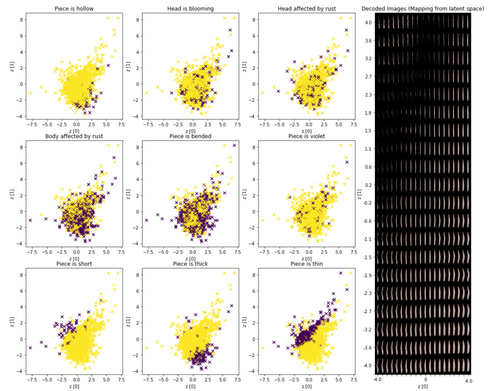
\includegraphics[scale=0.8]{Figures/chapter04/autoencoder}
	\decoRule
	\caption[??]{??}
	\label{fig:Autoencoder}
\end{figure}

It demonstrates that the features short thick and thin are mapped to separable clusters. As a tendency curvature correlates with a region in the lower periphery as indicated especially by the deconstruction. The other features (violet, rust and blooming) are not mapped adequately and they are not visible in the reconstruction. This shows that only some features of interest were mapped to the latent space and used to decode images. Reconstructions of autoencoders are known to miss many details. Better results could potentially have been achieved using larger input images. The possibility to generate, for example, more or less curved asparagus pieces may help to define a clear cut decision boundary and classify images accordingly. As a potential feature for asparagus sorting machines this would allow the user to customize the definition of curvature to his or her own taste. For this approach to be viable for all features, however, the network performance appears to be insufficient. Some features are poorly separated by our network that was employed on downscaled images.


\subsection{Semi-supervised learning}

We collected xxxx samples. With respect to the limited variance substantial amount of data. However, the target categories and information regarding the features present for each peace are unavailable. Labels had to be manually generated. Hence there is only a small subset of data where labels were attributed. A small amount of labeled data means that predictions can be successful only if there is little variance in the source values. Hence, for high dimensional data such as images sparse representations are desirable. A strategy that is especially appealing if large amounts of data are available is to automatically extract features instead of relying on feature engineering.
In the previous chapter methods for unsupervised learning were explained and the results for the given data presented. One example are autoencoders. Here we used convolutional autoencoders with additional soft constraints in the loss function for semi supervised learning. Instead of extracting features and then using the resulting sparse representation to train a machine learning classifier named technique relies on doing both at the same time: The strategy in semi supervised learning with bottleneck layer neural networks is simultaneously extracting features and enforcing that they (or at least some) correlate with the target categories. \\
The network: For the encoder a feedforward CNN was used that has proven to be suitable to detect at least some features with sufficient adequacy. ???????? layers…. NETWORK DETAILS. A challenge resulted from training with multiple inputs. As deep learning frameworks (here we employed Keras) usually require a connected graph that links inputs to outputs a trick was used. A dummy layer was introduced where all information that stems from the labels was multiplied by zero. The output vector was concatenated in the bottleneck of the encoder. As it contains no variance training and more importantly validation accuracies remain unaffected even though information about the categories that are predicted is added on the input side. The result is a few dead neurons only. For the decoder we chose the one of the variational autoencoder presented in the previous chapter. Two variations of the named network were tested: A convolutional variational autoencoder and a variational autoencoder for semi supervised learning.\\
A custom conditional loss function was used. If labels are present for the current batch a combined loss was used that comprised the reconstruction loss and the label loss. Here, reconstruction loss refers to the pixelwise loss that was used for the main task of the network  - namely mapping of input images back to the same input while the label loss is used with the goal of mapping label layer activations to the actual labels. It is low if activations in the sigmoid transformed label layer match the target values i.e. the sum of the error layer error layer is low. The loss that is due to labels was multiplied by a custom factor (k). In addition it was defined such that it scales with the current pixel wise reconstruction loss and converges to a constant (c). These values were chosen aiming for an increase of the contribution of the label loss to the combined loss especially in late stages of training.

\begin{figure}[h]
	\centering
	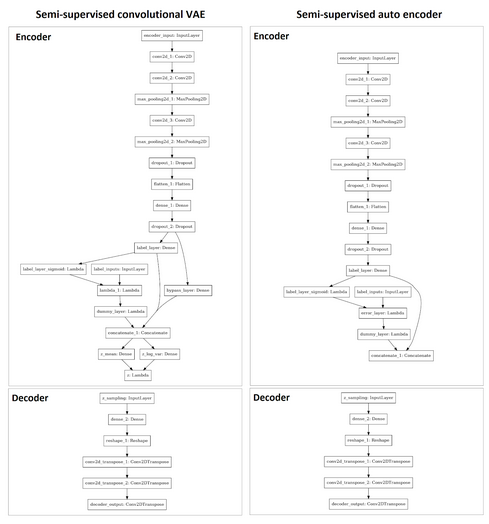
\includegraphics[scale=0.8]{Figures/chapter04/vae}
	\decoRule
	\caption[??]{??}
	\label{fig:VAE}
\end{figure}
\\
\begin{figure}[h]
	\centering
	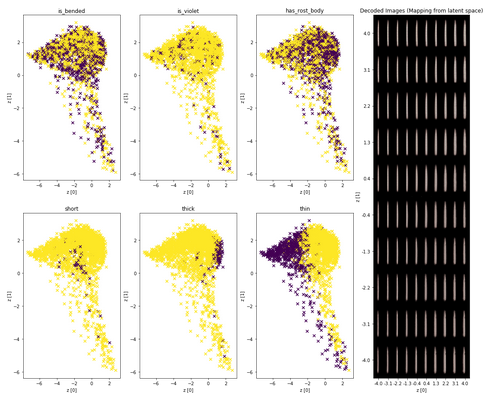
\includegraphics[scale=0.8]{Figures/chapter04/vae_2}
	\decoRule
	\caption[??]{??}
	\label{fig:VAE2}
\end{figure}
\\
\begin{figure}[h]
	\centering
	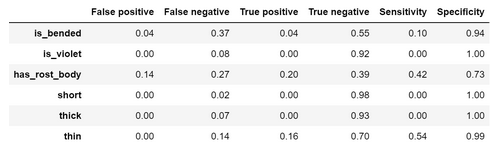
\includegraphics[scale=0.8]{Figures/chapter04/vae_table}
	\decoRule
	\caption[??]{??}
	\label{fig:VAEtable}
\end{figure}